\documentclass[tikz,border=8pt]{standalone}
\usetikzlibrary{arrows.meta,positioning,calc}
\begin{document}
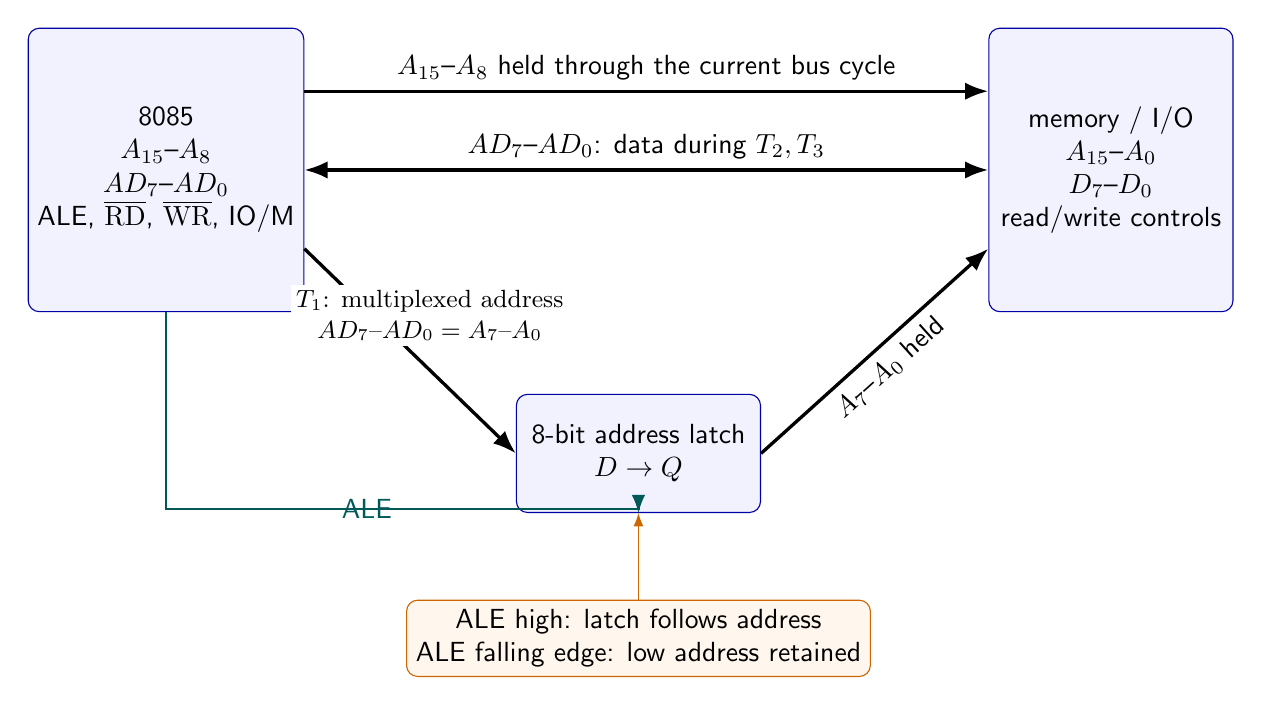
\begin{tikzpicture}[font=\sffamily,>=Latex,
blk/.style={draw=blue!65!black,rounded corners,fill=blue!5,minimum width=31mm,minimum height=15mm,align=center},
bus/.style={very thick,->},sig/.style={thick,->,teal!70!black}]
\node[blk,minimum height=36mm] (cpu) at (0,2) {8085\\$A_{15}$--$A_8$\\$AD_7$--$AD_0$\\ALE, $\overline{\rm RD}$, $\overline{\rm WR}$, IO/M};
\node[blk,minimum height=36mm] (dev) at (12,2) {memory / I/O\\$A_{15}$--$A_0$\\$D_7$--$D_0$\\read/write controls};
\node[blk] (latch) at (6,-1.6) {8-bit address latch\\$D\rightarrow Q$};
\draw[bus] ([yshift=10mm]cpu.east)--node[above]{$A_{15}$--$A_8$ held through the current bus cycle}([yshift=10mm]dev.west);
\draw[bus,<->] (cpu.east)--node[above]{$AD_7$--$AD_0$: data during $T_2,T_3$}(dev.west);
\draw[bus] ([yshift=-10mm]cpu.east)--(latch.west);
\node[fill=white,inner sep=2pt,font=\small,align=center] at (3.35,.15) {$T_1$: multiplexed address\\$AD_7$--$AD_0=A_7$--$A_0$};
\draw[bus] (latch.east)--node[below,sloped]{$A_7$--$A_0$ held}([yshift=-10mm]dev.west);
\draw[sig] (cpu.south)--++(0,-25mm)-|node[pos=.25,left]{ALE}(latch.south);
\node[below=11mm of latch,draw=orange!80!black,fill=orange!7,rounded corners,align=center] (phase) {ALE high: latch follows address\\ALE falling edge: low address retained};
\draw[->,orange!80!black] (phase)--(latch);
\end{tikzpicture}
\end{document}
